\section{Optional Extension: Subgraph Homomorphism}
\label{sec:optional-homomorphism}

The final optional extension implements subgraph \emph{homomorphism}, which relaxes the exact-matching semantics of the core reproduction in two ways. Given $G = (V_G, E_G, \ell_G)$ and $Q = (V_Q, E_Q, \ell_Q)$, a subgraph homomorphism is a map $f : V_Q \rightarrow V_G$ such that (a) labels are preserved, $\ell_Q(v) = \ell_G(f(v))$ for all $v$; (b) every query edge maps into the augmented edge set $E_G^+ = E_G \cup \{(w, w) : w \in V_G\}$, that is, $(u, v) \in E_Q \Rightarrow (f(u), f(v)) \in E_G^+$; and (c) $f$ need not be injective, so several query vertices may collapse onto the same data vertex. When endpoints collapse, the induced edge is a self-loop, which $E_G^+$ accepts uniformly, so no conflict arises. Concretely, a query edge $(u, v)$ is satisfied iff $f(u) = f(v)$ or $(f(u), f(v)) \in E_G$.

\subsection{Relationship to Subgraph Isomorphism}

Homomorphism is a strict relaxation of the isomorphism studied in the main report, and the two are connected by a clean identity. Every subgraph isomorphism is a homomorphism, because $E_G \subseteq E_G^+$ and injectivity is a special case. Conversely, because the query graph is loop-free, any two distinct query vertices joined by an edge must receive \emph{different} images under an injective map, so the self-loop case of $E_G^+$ never applies; an \emph{injective} homomorphism therefore satisfies $(f(u), f(v)) \in E_G$ for every query edge and is exactly a subgraph isomorphism. Hence
\[
\mathrm{Iso}(Q, G) \;=\; \{\, f \in \mathrm{Hom}(Q, G) : f \text{ is injective} \,\}, \qquad \mathrm{Iso}(Q, G) \subseteq \mathrm{Hom}(Q, G),
\]
and the additional homomorphisms are precisely the non-injective ones obtained by collapsing query vertices through self-loops. We use this identity as a built-in correctness oracle below.

\subsection{Algorithm}

The homomorphism matcher reuses the backtracking skeleton of the core reproduction with two principled changes. First, the injectivity check is removed: a data vertex may be assigned to more than one query vertex. Second, the edge-feasibility test is evaluated over $E_G^+$: when extending the current partial map with $f(q) = d$, for every already-mapped query neighbor $n$ the pair $(d, f(n))$ is accepted if $d = f(n)$ (a self-loop) or $(d, f(n)) \in E_G$.

A subtle but important consequence is that the label-and-degree (LDF) candidate filter used for isomorphism becomes \emph{unsound} for homomorphism. Because several query neighbors may map to the same data vertex---or to $f(q)$ itself via a self-loop---a low-degree or even isolated data vertex can legitimately host a high-degree query vertex. The matcher therefore uses \emph{label-only} candidates. The reference implementation is \texttt{src/subgraph\_match/homomorphism/} with the experiment harness in \texttt{scripts/run\_homomorphism\_experiment.py}.

\subsection{Correctness Validation}

Correctness is verified at three levels in \texttt{tests/test\_homomorphism\_matcher.py}. First, the matcher output is compared against an independent brute-force oracle that enumerates \emph{all} label-respecting functions $V_Q \rightarrow V_G$ and tests the $E_G^+$ edge constraint directly, on the toy graph and on small cliques. Second, the identity above is checked: the injective subset of the homomorphism results equals the isomorphism results returned by the baseline matcher, and the isomorphisms form a subset of the homomorphisms. Third, edge cases are covered, including collapsing two non-adjacent vertices through a self-loop and mapping an entire triangle query onto a single isolated data vertex (which an unsound degree filter would wrongly reject). All experiments below also report these cross-checks.

\subsection{Experimental Results}

Table~\ref{tab:homomorphism} reports homomorphism counts against isomorphism counts. ``Toy'' uses the $A\!-\!A$ edge query on the debugging graph. ``Hom-demo'' is a deterministic synthetic graph (\texttt{scripts/make\_homomorphism\_demo\_graph.py}) consisting of $15$ disjoint cliques of size $6$, all labeled $A$, queried with the triangle $A\!-\!A\!-\!A$; per clique every one of the $6^3$ vertex assignments is a homomorphism while only $6\cdot 5\cdot 4$ are isomorphisms.

\begin{table*}[t]
  \caption{Subgraph homomorphism vs.\ subgraph isomorphism. ``Injective Hom'' is the injective subset of the homomorphisms and must equal ``Iso''. ``Non-inj.\ Hom'' are the additional non-injective homomorphisms. ``Hom PM'' is the partial mappings explored by the homomorphism search.}
  \label{tab:homomorphism}
  \centering
  \small
  \begin{tabular}{llrrrrrrc}
    \toprule
    Dataset & Query & Hom & Iso & Injective Hom & Non-inj.\ Hom & Hom PM & Hom (ms) & Inj.\ Hom $=$ Iso \\
    \midrule
    Toy & $A\!-\!A$ & 4 & 2 & 2 & 2 & 6 & 0.009 & yes \\
    Hom-demo & $A\!-\!A\!-\!A$ & 3{,}240 & 1{,}800 & 1{,}800 & 1{,}440 & 3{,}870 & 12.32 & yes \\
    \bottomrule
  \end{tabular}
\end{table*}

\begin{figure}[t]
  \centering
  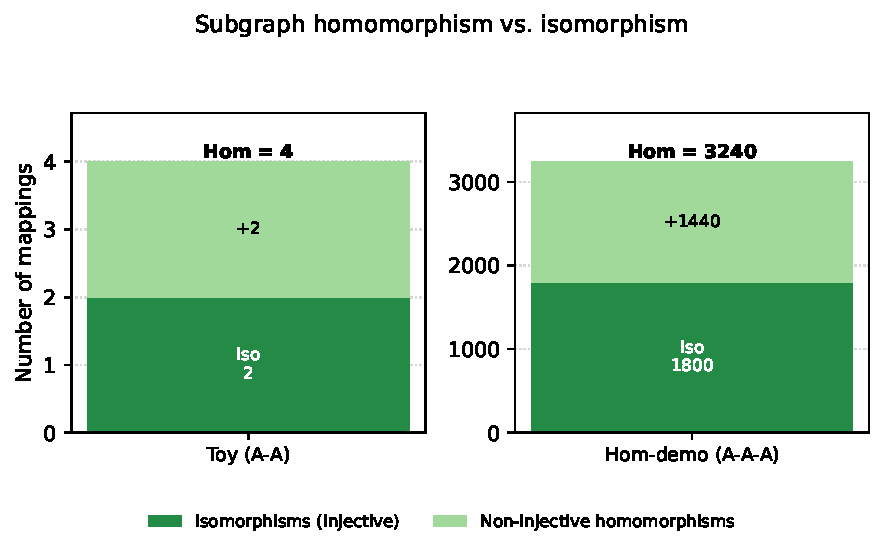
\includegraphics[width=0.72\linewidth]{figures/homomorphism.pdf}
  \caption{Homomorphism counts decompose into the injective part (which equals the isomorphism count) and the additional non-injective homomorphisms produced by the $E_G^+$ self-loop relaxation. Source: \texttt{reports/figures/plot\_homomorphism.py} (data \texttt{homomorphism\_data.csv}).}
  \label{fig:homomorphism}
\end{figure}

The results confirm the theory (Figure~\ref{fig:homomorphism}). In every case the injective subset of the homomorphisms equals the isomorphisms exactly ($2$ on the toy graph, $1{,}800$ on the demo), validating both the homomorphism matcher and, independently, the baseline isomorphism matcher. The relaxation is far from cosmetic: on the toy graph the two non-injective homomorphisms collapse the $A\!-\!A$ query onto a single $A$ vertex through the self-loop, and on the demo the self-loop relaxation produces $1{,}440$ additional homomorphisms on top of the $1{,}800$ isomorphisms ($3{,}240 = 15 \cdot 6^3$ total). Because homomorphism enumerates strictly more mappings and cannot use degree pruning, its search is somewhat heavier than the isomorphism search ($12.32$\,ms vs.\ the baseline's $11.14$\,ms on the demo), which is the expected cost of the broader solution space. This extension is restricted to vertex-labeled, loop-free queries and reuses the same label-only candidate model throughout; combining it with the guard-based pruning of the core reproduction is left as future work.
